% The San Francisco Social Media Data and Analytics Group
% 05 November 2013
% Scott Hendrickson
% @DrSkippy27
% Gnip

\documentclass{beamer}
\setbeamertemplate{navigation symbols}{}

% THEMES
\usetheme{gnip}
% PACKAGES
\usepackage[group-separator={,}]{siunitx}
%\usepackage{fontspec}
\usepackage{graphicx}
% FOOTER
\setbeamertemplate{footline}[text line]{
\colorbox{white}{\parbox[22px]{\paperwidth} {\color{linecolour} {\line(1,0){500} \\ \hfill @DrSkippy27 @gnip}}}
}
\beamersetuncovermixins{\opaqueness<1>{25}}{\opaqueness<2->{15}}

\usepackage{minted}
\usepackage{tikz}

\begin{document}
\title{Data Scientist's Approach to Social Data}
\author{Scott Hendrickson \\ Principal Data Scientist, Gnip \\  @DrSkippy27}
\date{\today} 

% title

\begin{frame}
\titlepage
\end{frame}

%%%%%%%%
\section{Social Data}

\begin{frame}\frametitle{Social Data}
\begin{center}
{\Huge created by \\ [8pt] interactions \\ [15pt] among people}
\end{center}
\end{frame}

\begin{frame}\frametitle{Social Data}
\begin{center}
{\Huge form and content \\ [8pt] shaped by \\ [15pt] people}
\end{center}
\end{frame}

\begin{frame}\frametitle{Sources of Social Data}
{\Huge
\begin{itemize}
\item Firehoses
\item APIs
\item Scraping
\end{itemize}
}
\end{frame}

% Firehoses

\subsection{Firehose}

\begin{frame}\frametitle{Firehose}
\begin{center}
{\Huge Continuous stream \\ [8pt] of activities \\ [15pt] in near-real time}
\end{center}
\end{frame}

% Activity 

\begin{frame}\frametitle{Social Data Activity}
\begin{center}
{\Huge People interact \\ [8pt] on social media platform}
\end{center}
\end{frame}

% Volumes

\begin{frame} \frametitle{Firehose volumes}
\begin{table}
\begin{tabular}{l|r}
\hline
   {Publisher}   &   {Daily Activity}   \\
\hline 
    Twitter      &      500M   \\
    Tumblr      &       105M   \\
    Foursquare &       4.3M \\
    GetGlue &         430k \\
    Wordpress Posts &     919k   \\
    Wordpress Comments & 1.7M \\
    Disqus       &       1.9M  \\
    Engagement (likes, votes) & 59M  \\
\hline
\end{tabular}
\end{table}
\end{frame}

%

\begin{frame}\frametitle{Daily @Gnip}
\begin{center}
{\Huge $\frac{3}{4}$ Billion IN \\ [18pt] 4 Billion OUT}
\end{center}
\end{frame}

% Source considerations

\begin{frame}\frametitle{Analysis Considerations}
{\Large
\begin{itemize}
\item Technology - interfaces, tools, infrastructure for accessing
\item Latency - how soon after activity as created?
\item Uniformity - how hard/costly to normalize data formats?
\item Coverage - do you need it all? a defined sample?
\item Meta-data -  how much and what kind of data about the data?
\end{itemize}
}
\end{frame}

% Source considerations

\begin{frame}\frametitle{Business Considerations}
{\Large
\begin{itemize}
\item Licensing - do you have the right to analyze, display, store data?
\item Terms-of-Service Compliance - violating publishers terms of service, privacy protections?
\item Cost - data collection costs? licensing costs? processing and storage costs?
\item Analysis mode - batch vs. real-time? event vs. background? time, structure, language, people?
\end{itemize}
}
\end{frame}


%%%%%%%%
\section{Analysis}

% what are we doing?

% models drive analysis ; analysis drives model picture

\begin{frame}\frametitle{Models}
\begin{itemize}
\item Model domain - timeseries, language analysis, network structures
\item Model domain drives storage/access strategy - test files, spreadsheets, relational dbs, no-sql dbs...
\item Analysis - dashboard vs. discovery projects
\end{itemize}
\end{frame}

% mind graph goes here!!!

%%%%%%%%
%%
%%  EXAMPLES
%%
%%%%%%%%


%%%%%%%%
\section{Time series - Social medial pulse}

% social media pulse

\section{Social media pulse}

% find dates, names

\begin{frame}\frametitle{Expected: Hurricane}
  \begin{center}
    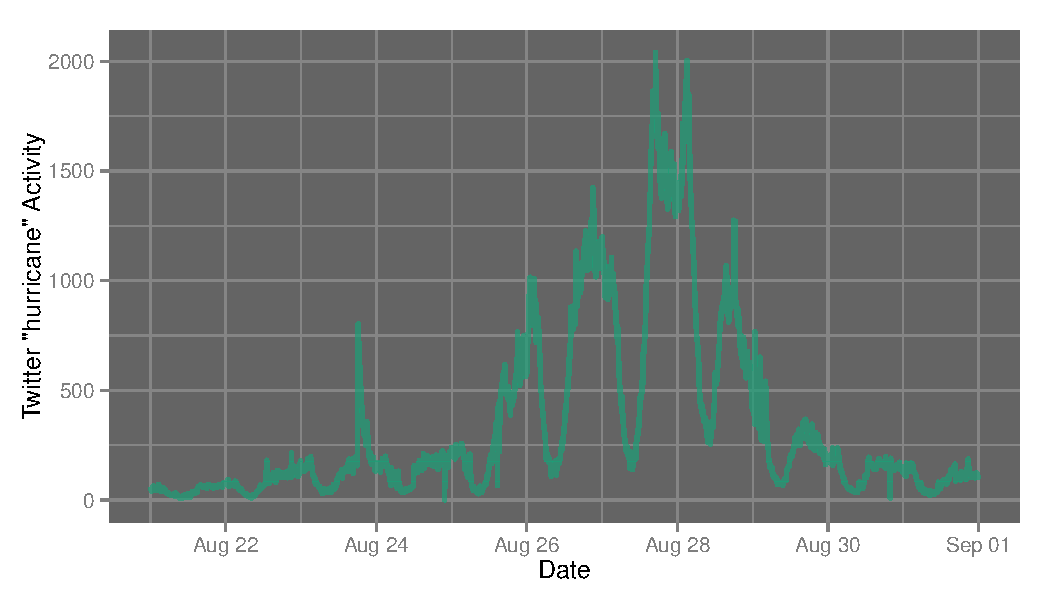
\includegraphics[width=11cm]{./imgs/SMP_hurricane.pdf}
  \end{center}
\end{frame}

\begin{frame}\frametitle{Unexpected: Earthquake}
  \begin{center}
    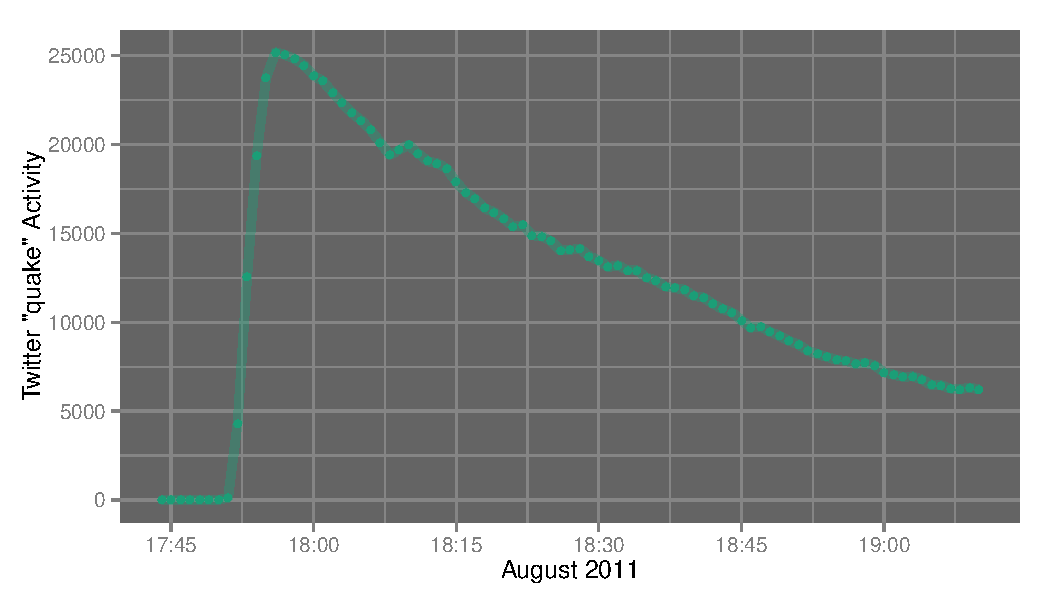
\includegraphics[width=11cm]{./imgs/SMP_va_quake.pdf}
  \end{center}
\end{frame}


% Events

\begin{frame}\frametitle{Classifying Events}
\begin{table}
\begin{tabular}{ m{2cm} | m{ 2.5cm} | m{4cm}}
\hline
Type & Response & Examples \\ \hline
Expected    & Approx. \newline Symmetric & Hurricane Sandy \newline Olympics \\ \hline
Unexpected (many obs.) & Social Media \newline Pulse & Beyonc\'{e} VMAs \newline  Mexico earthquake \newline  Steve Jobs \\ \hline
Unexpected  (network spread) \newline Models & Osama bin Laden \newline  Whitney Houston \newline  Syrian dissidents \\ \hline
\end{tabular}
\end{table}
\end{frame}


\begin{frame}\frametitle{Expected: Hurricane}
  \begin{center}
    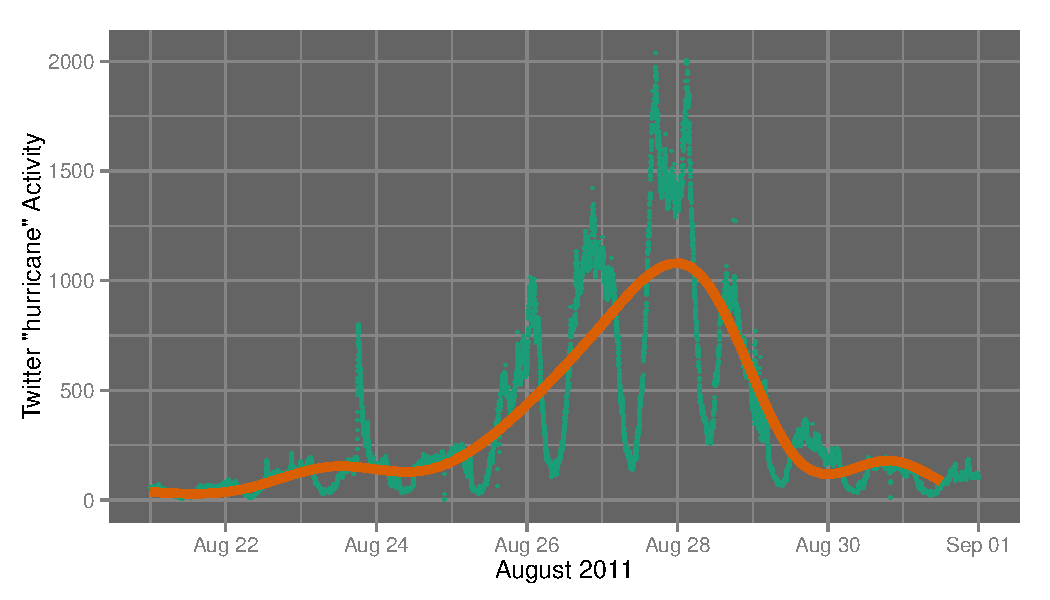
\includegraphics[width=11cm]{./imgs/SMP_hurricane_trend.pdf}
  \end{center}
\end{frame}


% half life

\begin{frame}\frametitle{Half-life}
\begin{center}
{\Huge time to observe \\[6pt] $\frac{1}{2}$ of the activities \\[6pt] for an event}
\end{center}
\end{frame}

\begin{frame}
\frametitle{Social media pulse} 
Given an event, the probability of a activity from one person,

\begin{equation*}
f(t) = \lambda \exp(-\lambda t), \text{ for } t \geq 0.
\end{equation*}

Many people posting, so sum of random variables $S = X_1 + X_2 + \ldots + X_{n \text{ posters}}$.

Probability distribution function,

\begin{equation*}
f_S(t) = \frac{ \beta^{-\alpha} t^{\alpha-1} \exp( \frac{-t}{\beta}) } {\Gamma(\alpha)}
\end{equation*}

Cumulative distribution is the ``generalized regularized incomplete gamma function'',

\begin{equation*}
F_S(t) = Q(\alpha, 0, \frac{ t}{\beta})
\end{equation*}
\end{frame}

% gamma plots

\begin{frame}
  \begin{center}
   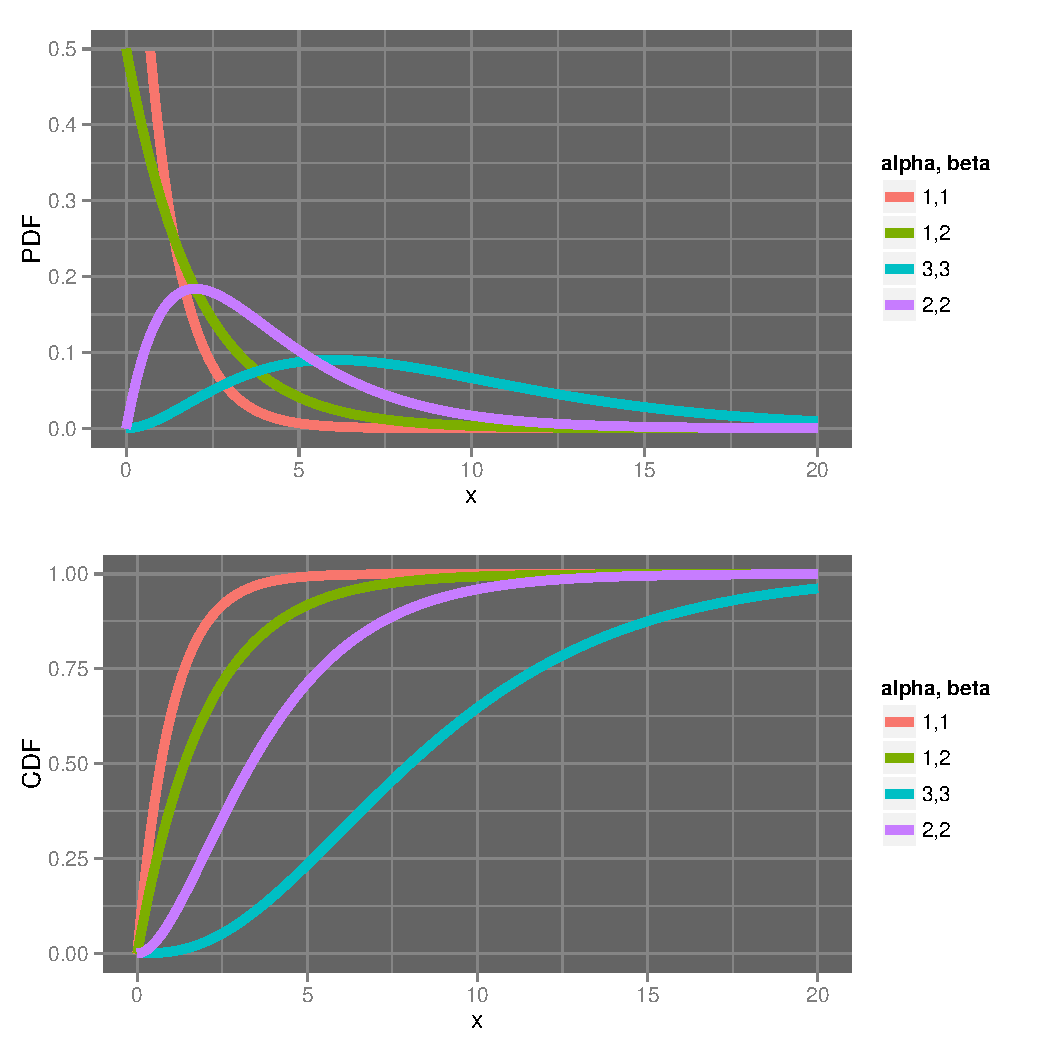
\includegraphics[height=6cm]{./imgs/SMP_gammadist.pdf}
  \end{center}
\end{frame}

\begin{frame}\frametitle{Why model half-life?}
\begin{center}
\begin{itemize}
\Huge{
\item predict total story volume
\item compare half-lives
\item anomalous story evolution
}
\end{itemize}
\end{center}
\end{frame}

\begin{frame}
  \begin{center}
    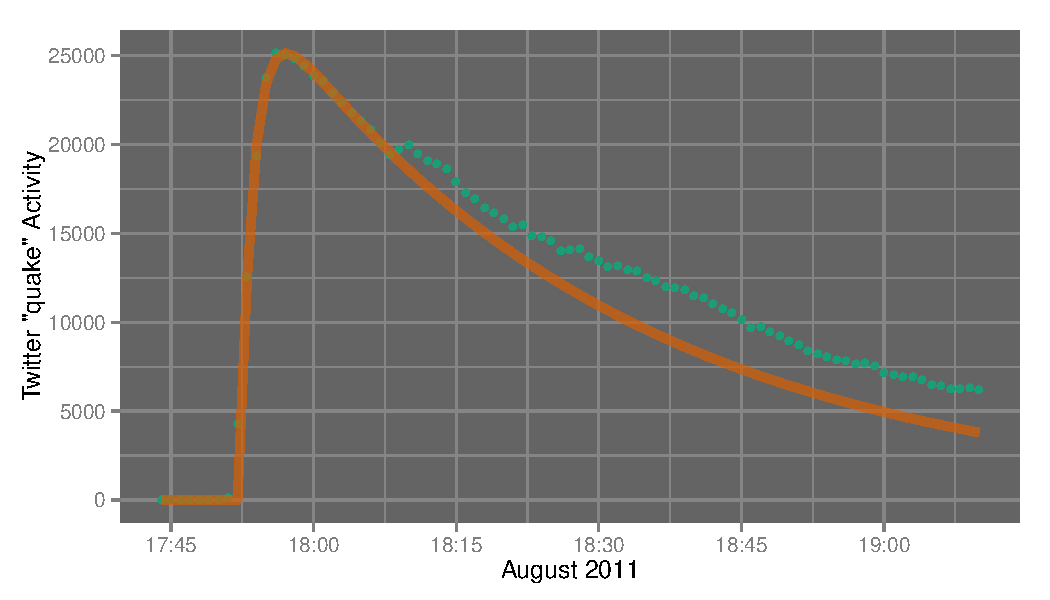
\includegraphics[width=8cm]{./imgs/SMP_va_quake_fit1.pdf}
  \end{center}
\end{frame}

% JPMorgan

\begin{frame}
  \begin{center}
    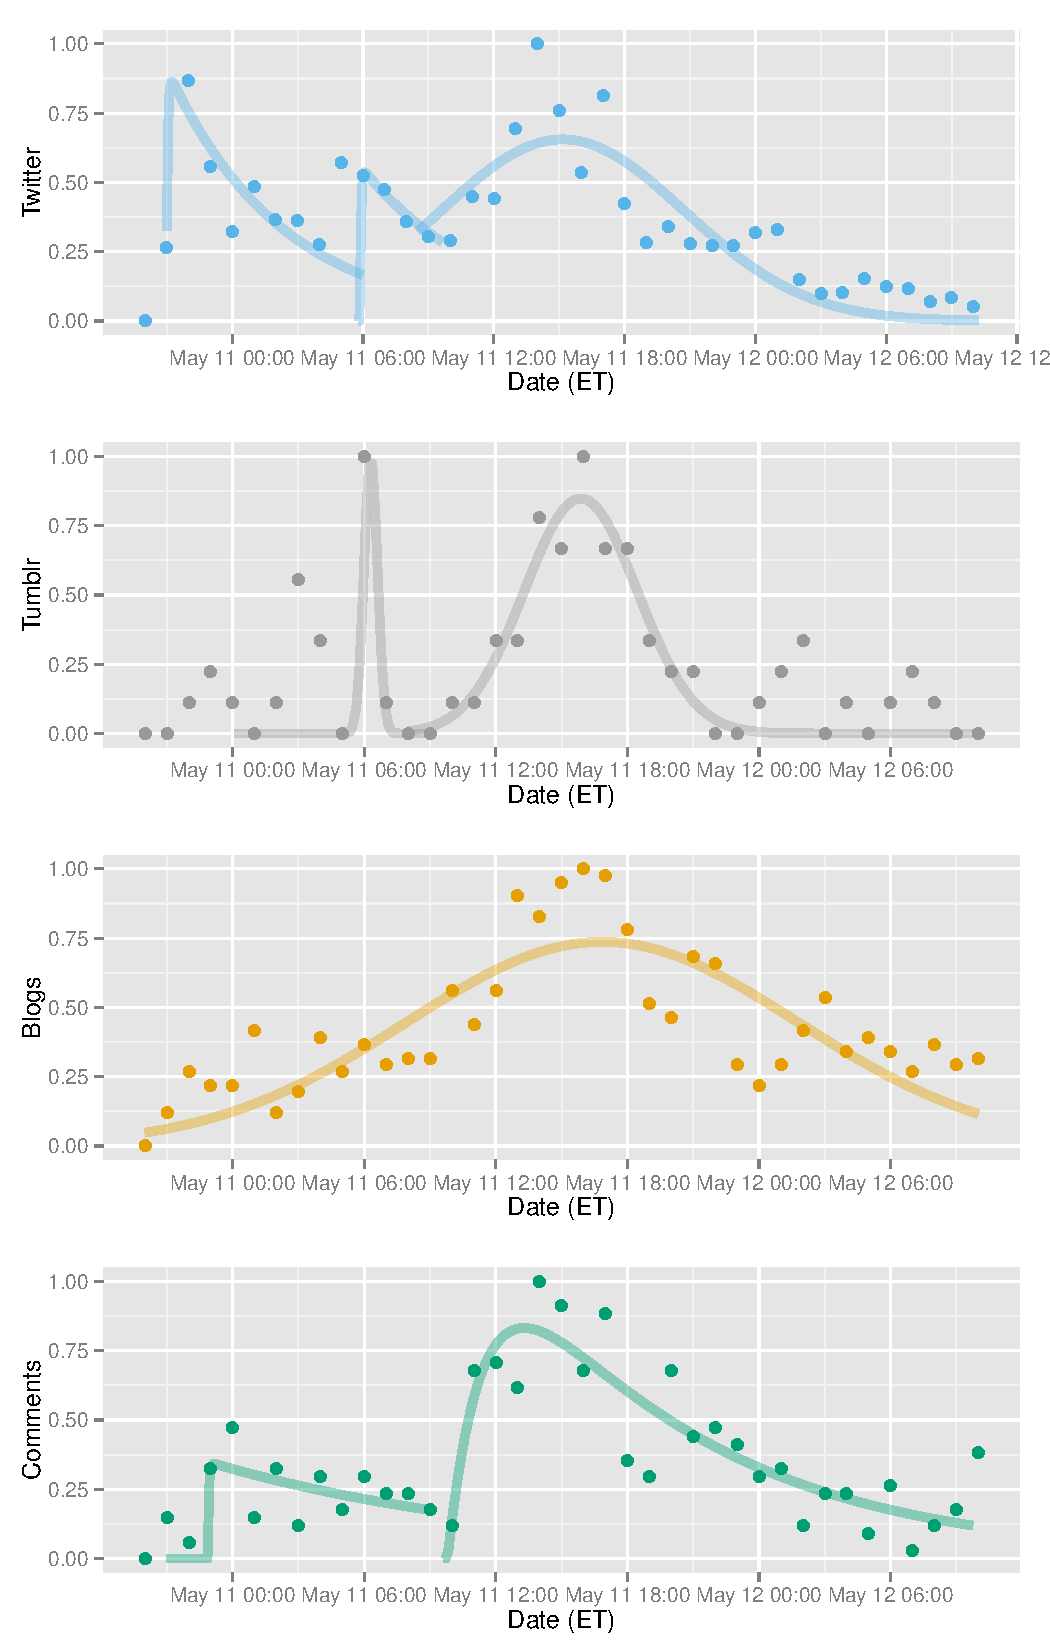
\includegraphics[height=8.5cm]{./imgs/SMP_JPMorgan.pdf}
  \end{center}
\end{frame}


%%%%%%%%
\section{Synthesis - Isreal and Hamas in Gaza}

\begin{frame}\frametitle{Comments with key words over time}
  \begin{center}
    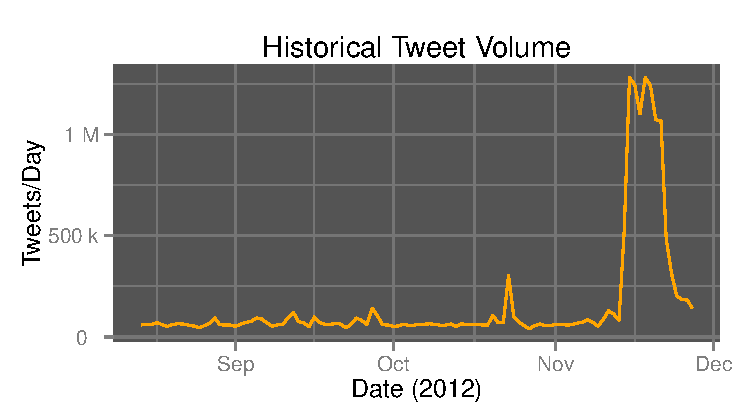
\includegraphics[width=9.5cm]{./imgs/HI_minimal-all-daily.pdf}
  \end{center}
\end{frame}

\begin{frame}\frametitle{Comments with key words over time}
  \begin{center}
    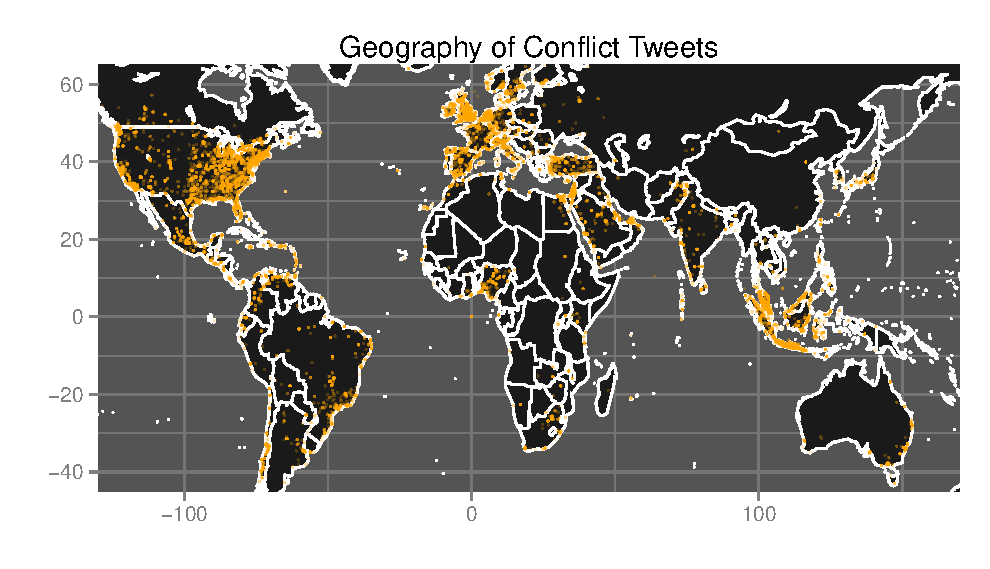
\includegraphics[width=9.5cm]{./imgs/HI_minimal-target-geo.pdf}
  \end{center}
\end{frame}

\begin{frame}\frametitle{Comments with key words over time}
  \begin{center}
    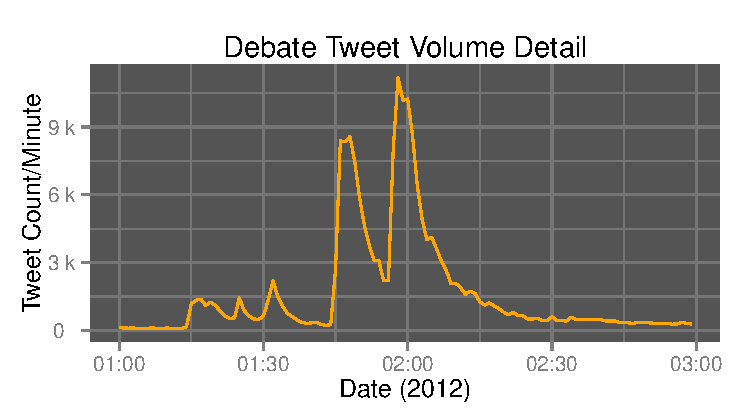
\includegraphics[width=9.5cm]{./imgs/HI_minimal-leadup-pres-debate.pdf}
  \end{center}
\end{frame}

\begin{frame}\frametitle{Comments with key words over time}
  \begin{center}
    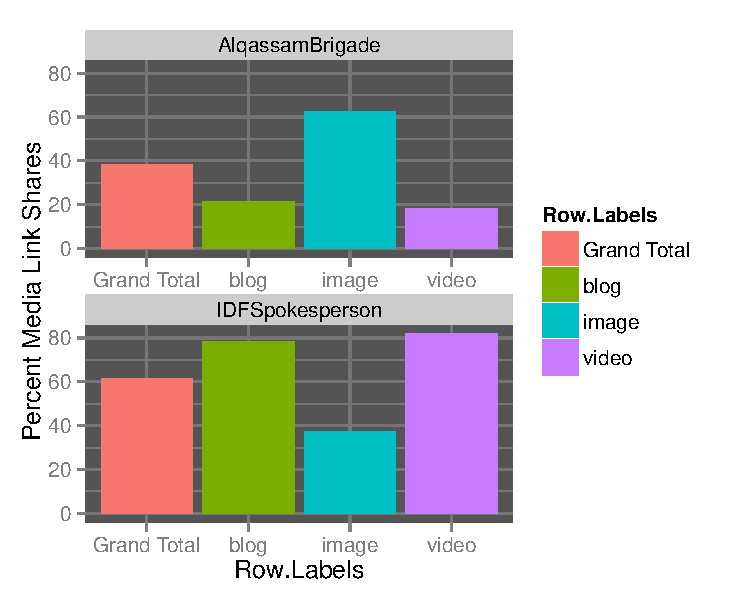
\includegraphics[width=9.5cm]{./imgs/HI_minimal-media.pdf}
  \end{center}
\end{frame}

\begin{frame}\frametitle{Comments with key words over time}
  \begin{center}
    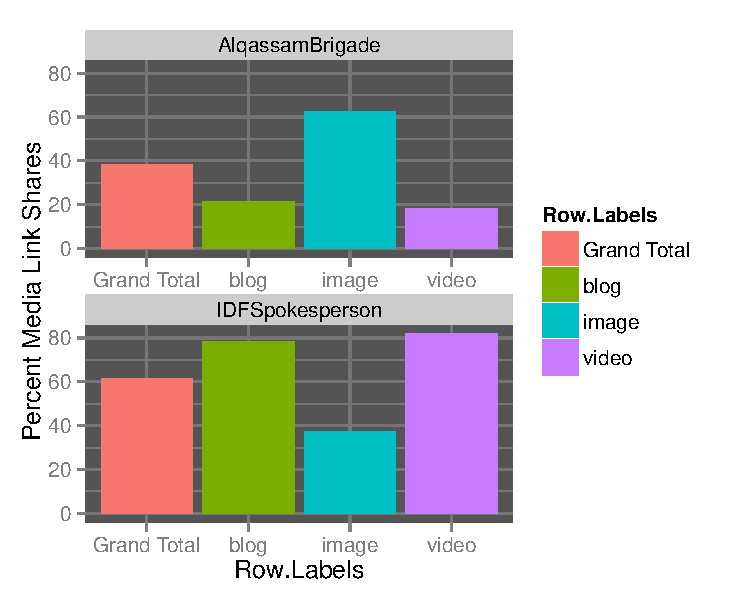
\includegraphics[width=9.5cm]{./imgs/HI_minimal-media.pdf}
  \end{center}
\end{frame}

\begin{frame}\frametitle{Comments with key words over time}
  \begin{center}
    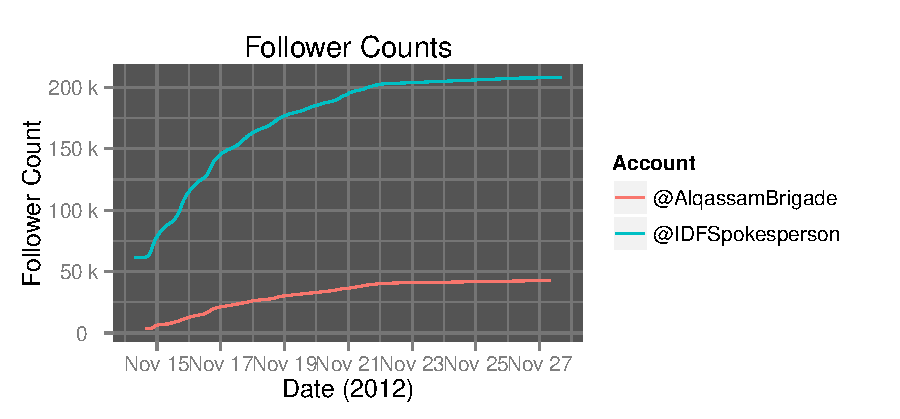
\includegraphics[width=9.5cm]{./imgs/HI_minimal-followers.pdf}
  \end{center}
\end{frame}


\begin{frame}\frametitle{Comments with key words over time}
  \begin{center}
    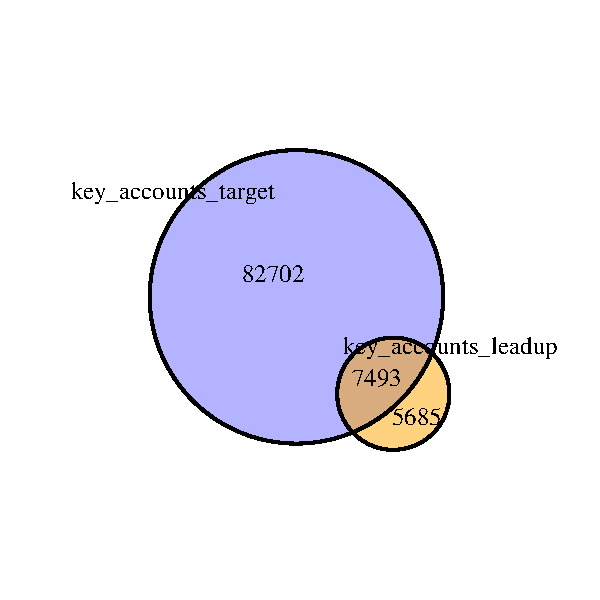
\includegraphics[width=9.5cm]{./imgs/HI_minimal-venns6.pdf}
  \end{center}
\end{frame}

\begin{frame}\frametitle{Comments with key words over time}
  \begin{center}
    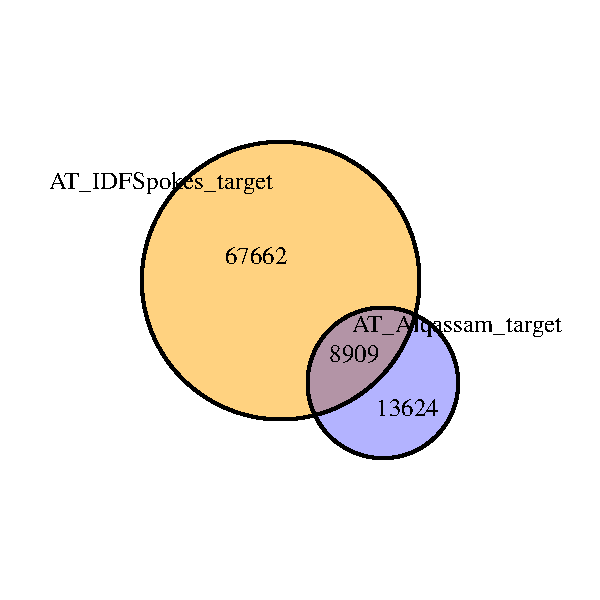
\includegraphics[width=9.5cm]{./imgs/HI_minimal-venns8.pdf}
  \end{center}
\end{frame}



%%%%%%%%
\section{Engagement is the Message}

%%%%%%%%
\section{Structure - Comments, Retweets, Replogs}

%%%%%%%%
\section{Self Selecting Audiences - Toyota}

% toyota
\begin{frame}
  \begin{center}
    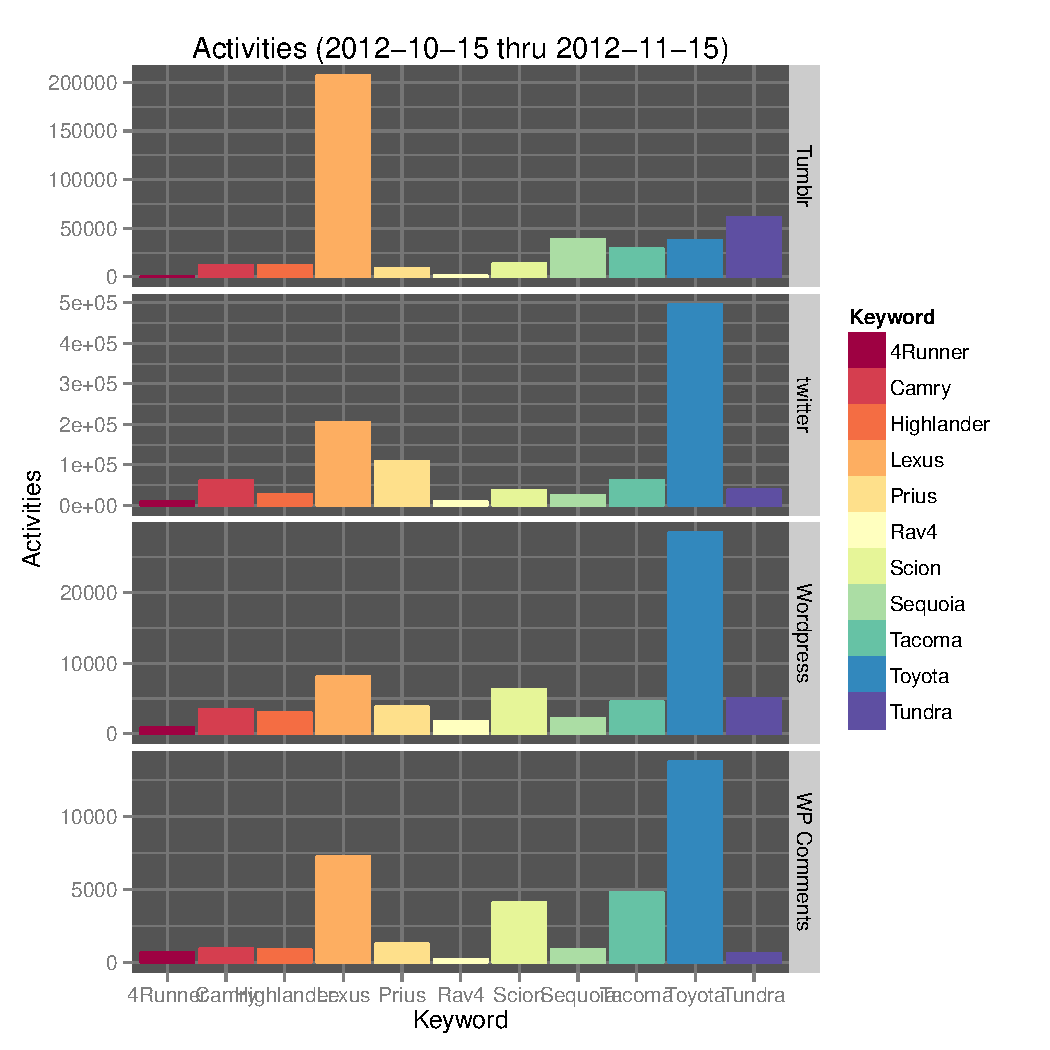
\includegraphics[width=8cm]{./imgs/TOY_bars.pdf}
  \end{center}
\end{frame}

%%%%%%%%
\section{Structure and Language - Topic Modeling}
% Raymond Carver, Bullwinkle and Rocky

\begin{frame}
\begin{center}
{\Huge What do we talk about \\ [15pt] when they talk about X?} 
\end{center}
\hfill Apologies: Raymond Carver \\
\end{frame}

\begin{frame}\frametitle{Disqus Tree Structures}
\begin{center}
{\Huge articles $\leftarrow$ comments \\ [20 pt] comments $\leftarrow$ comments}
\end{center}
\end{frame}

\begin{frame}\frametitle{Disqus Threads}
\begin{center}
{\Large 
\begin{enumerate}
\item 7 weeks
\item Key words: ``texting,'' ``driving'' and variants
\item Select top threads based on mentions
\item 61,406 comments from 365 threads
\end{enumerate}
}
\end{center}
\end{frame}

\begin{frame}\frametitle{Disqus Topic Model Approach}
\begin{center}
{\Large 
\begin{enumerate}
\item Find comments that mention key words
\item Corpus of comments (across many threads)
\item tf-idf matrix: terms $\times$ comments
\item LSI (rotate space to align with ``important'' dimensions, cut dimensions)
\item K-means (quick-and-dirty clustering in reduced dimensional space)
\item \ldots rinse and repeat (looking for distinction and cohesion)
\end{enumerate}
}
\end{center}
\end{frame}

\begin{frame}\frametitle{Disqus Topic Model}
\begin{center}
{\Large 
\begin{enumerate}
\item Same 7 weeks; same keywords
\item 32,856 comments from 16,886 threads
\item LSI: 500 features $\rightarrow$ 80 features
\item K-means: 80 clusters as topics (?!)
\end{enumerate}
}
\end{center}
\end{frame}

\begin{frame}
\begin{center}
{\Huge Focus on the intersection of \\[15 pt] Thread and Topic models}
\end{center}
\end{frame}

%\begin{frame}\frametitle{Comments with key words over time}
%  \begin{center}
%    \includegraphics[width=9.5cm]{./imgs/time.pdf}
%  \end{center}
%\end{frame}

\begin{frame}\frametitle{Disqus Thread Activity over Time}
  \begin{center}
    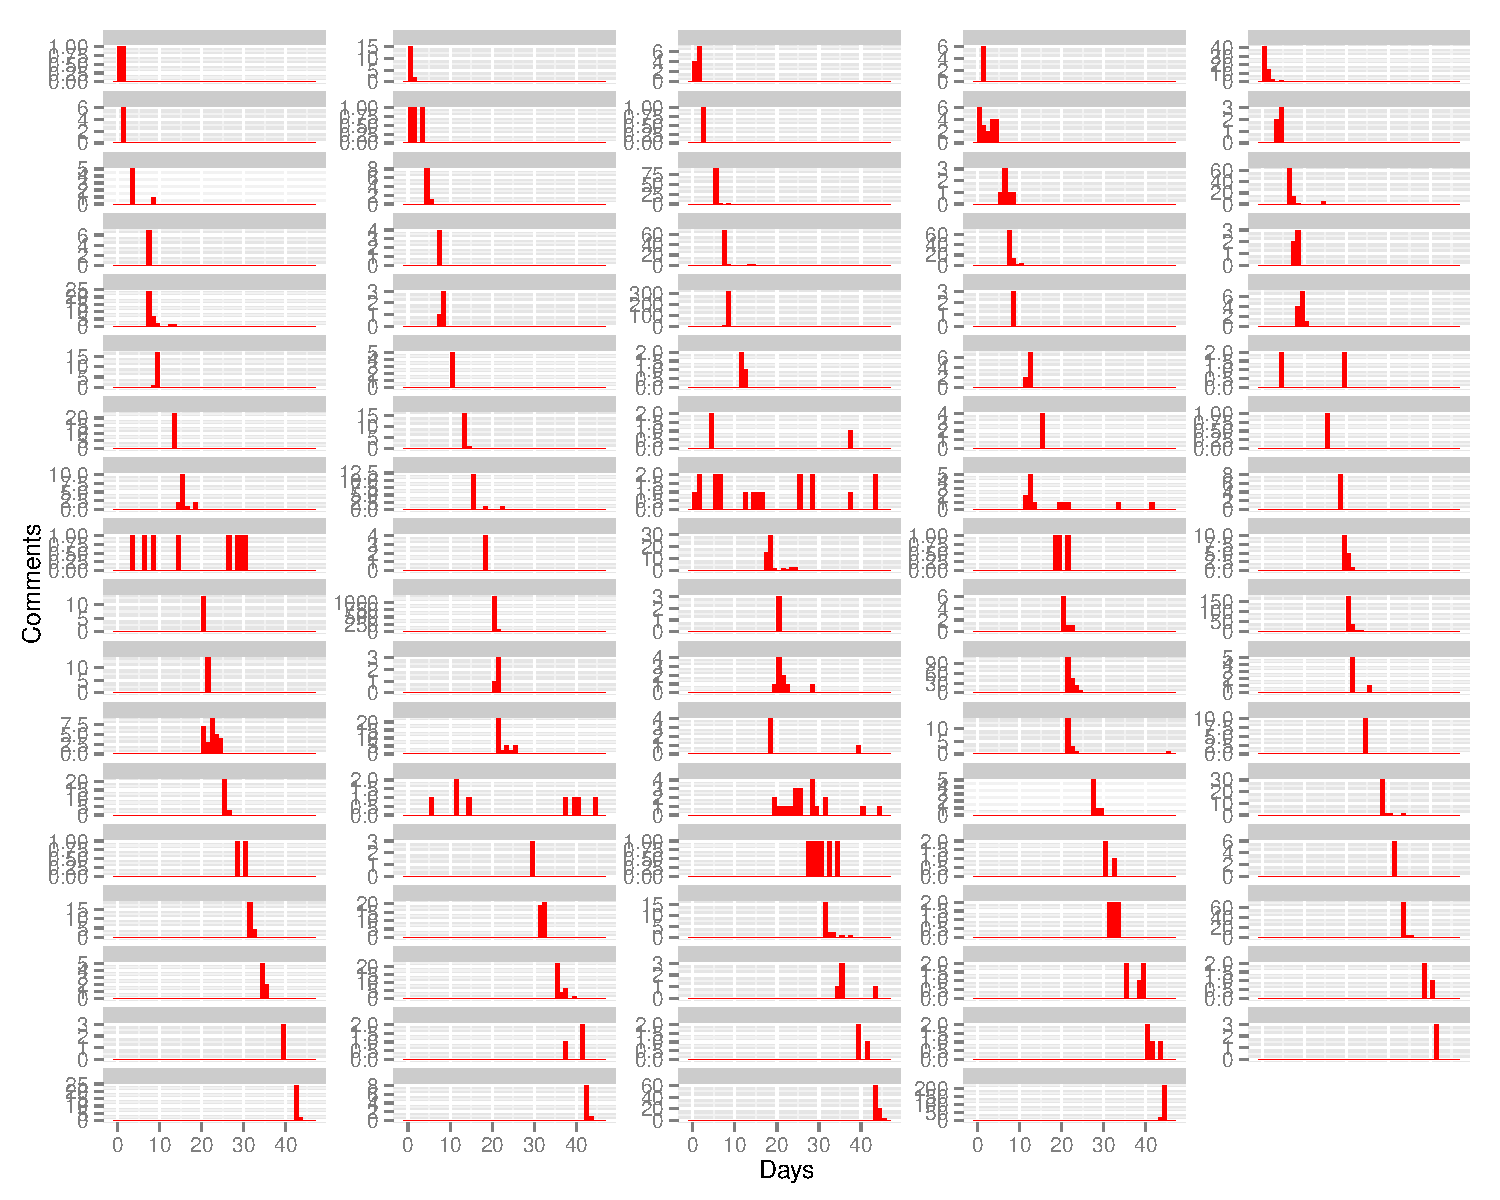
\includegraphics[width=9.5cm]{./imgs/DT_timebythread.pdf}
  \end{center}
\end{frame}

\begin{frame}\frametitle{Disqus Topics Activity over Time}
  \begin{center}
    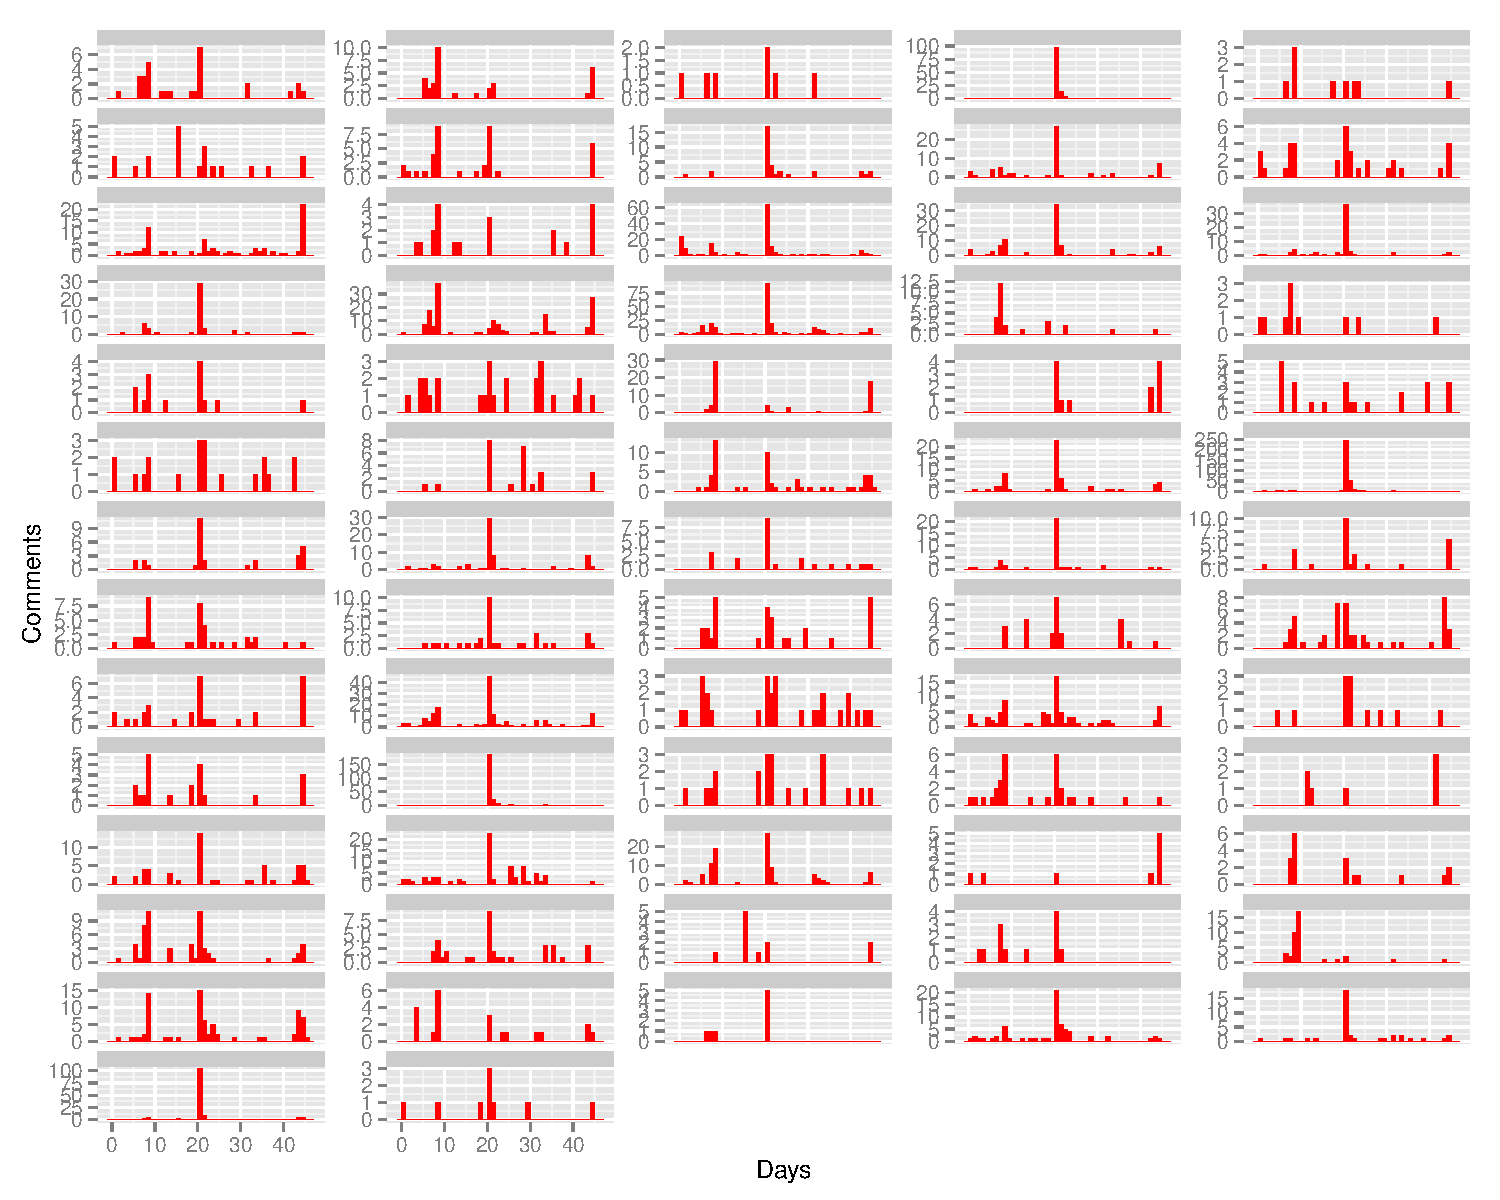
\includegraphics[width=9.5cm]{./imgs/DT_timebycluster.pdf}
  \end{center}
\end{frame}

\begin{frame}\frametitle{Dominant Topics $\times$ Threads?}
  \begin{center}
    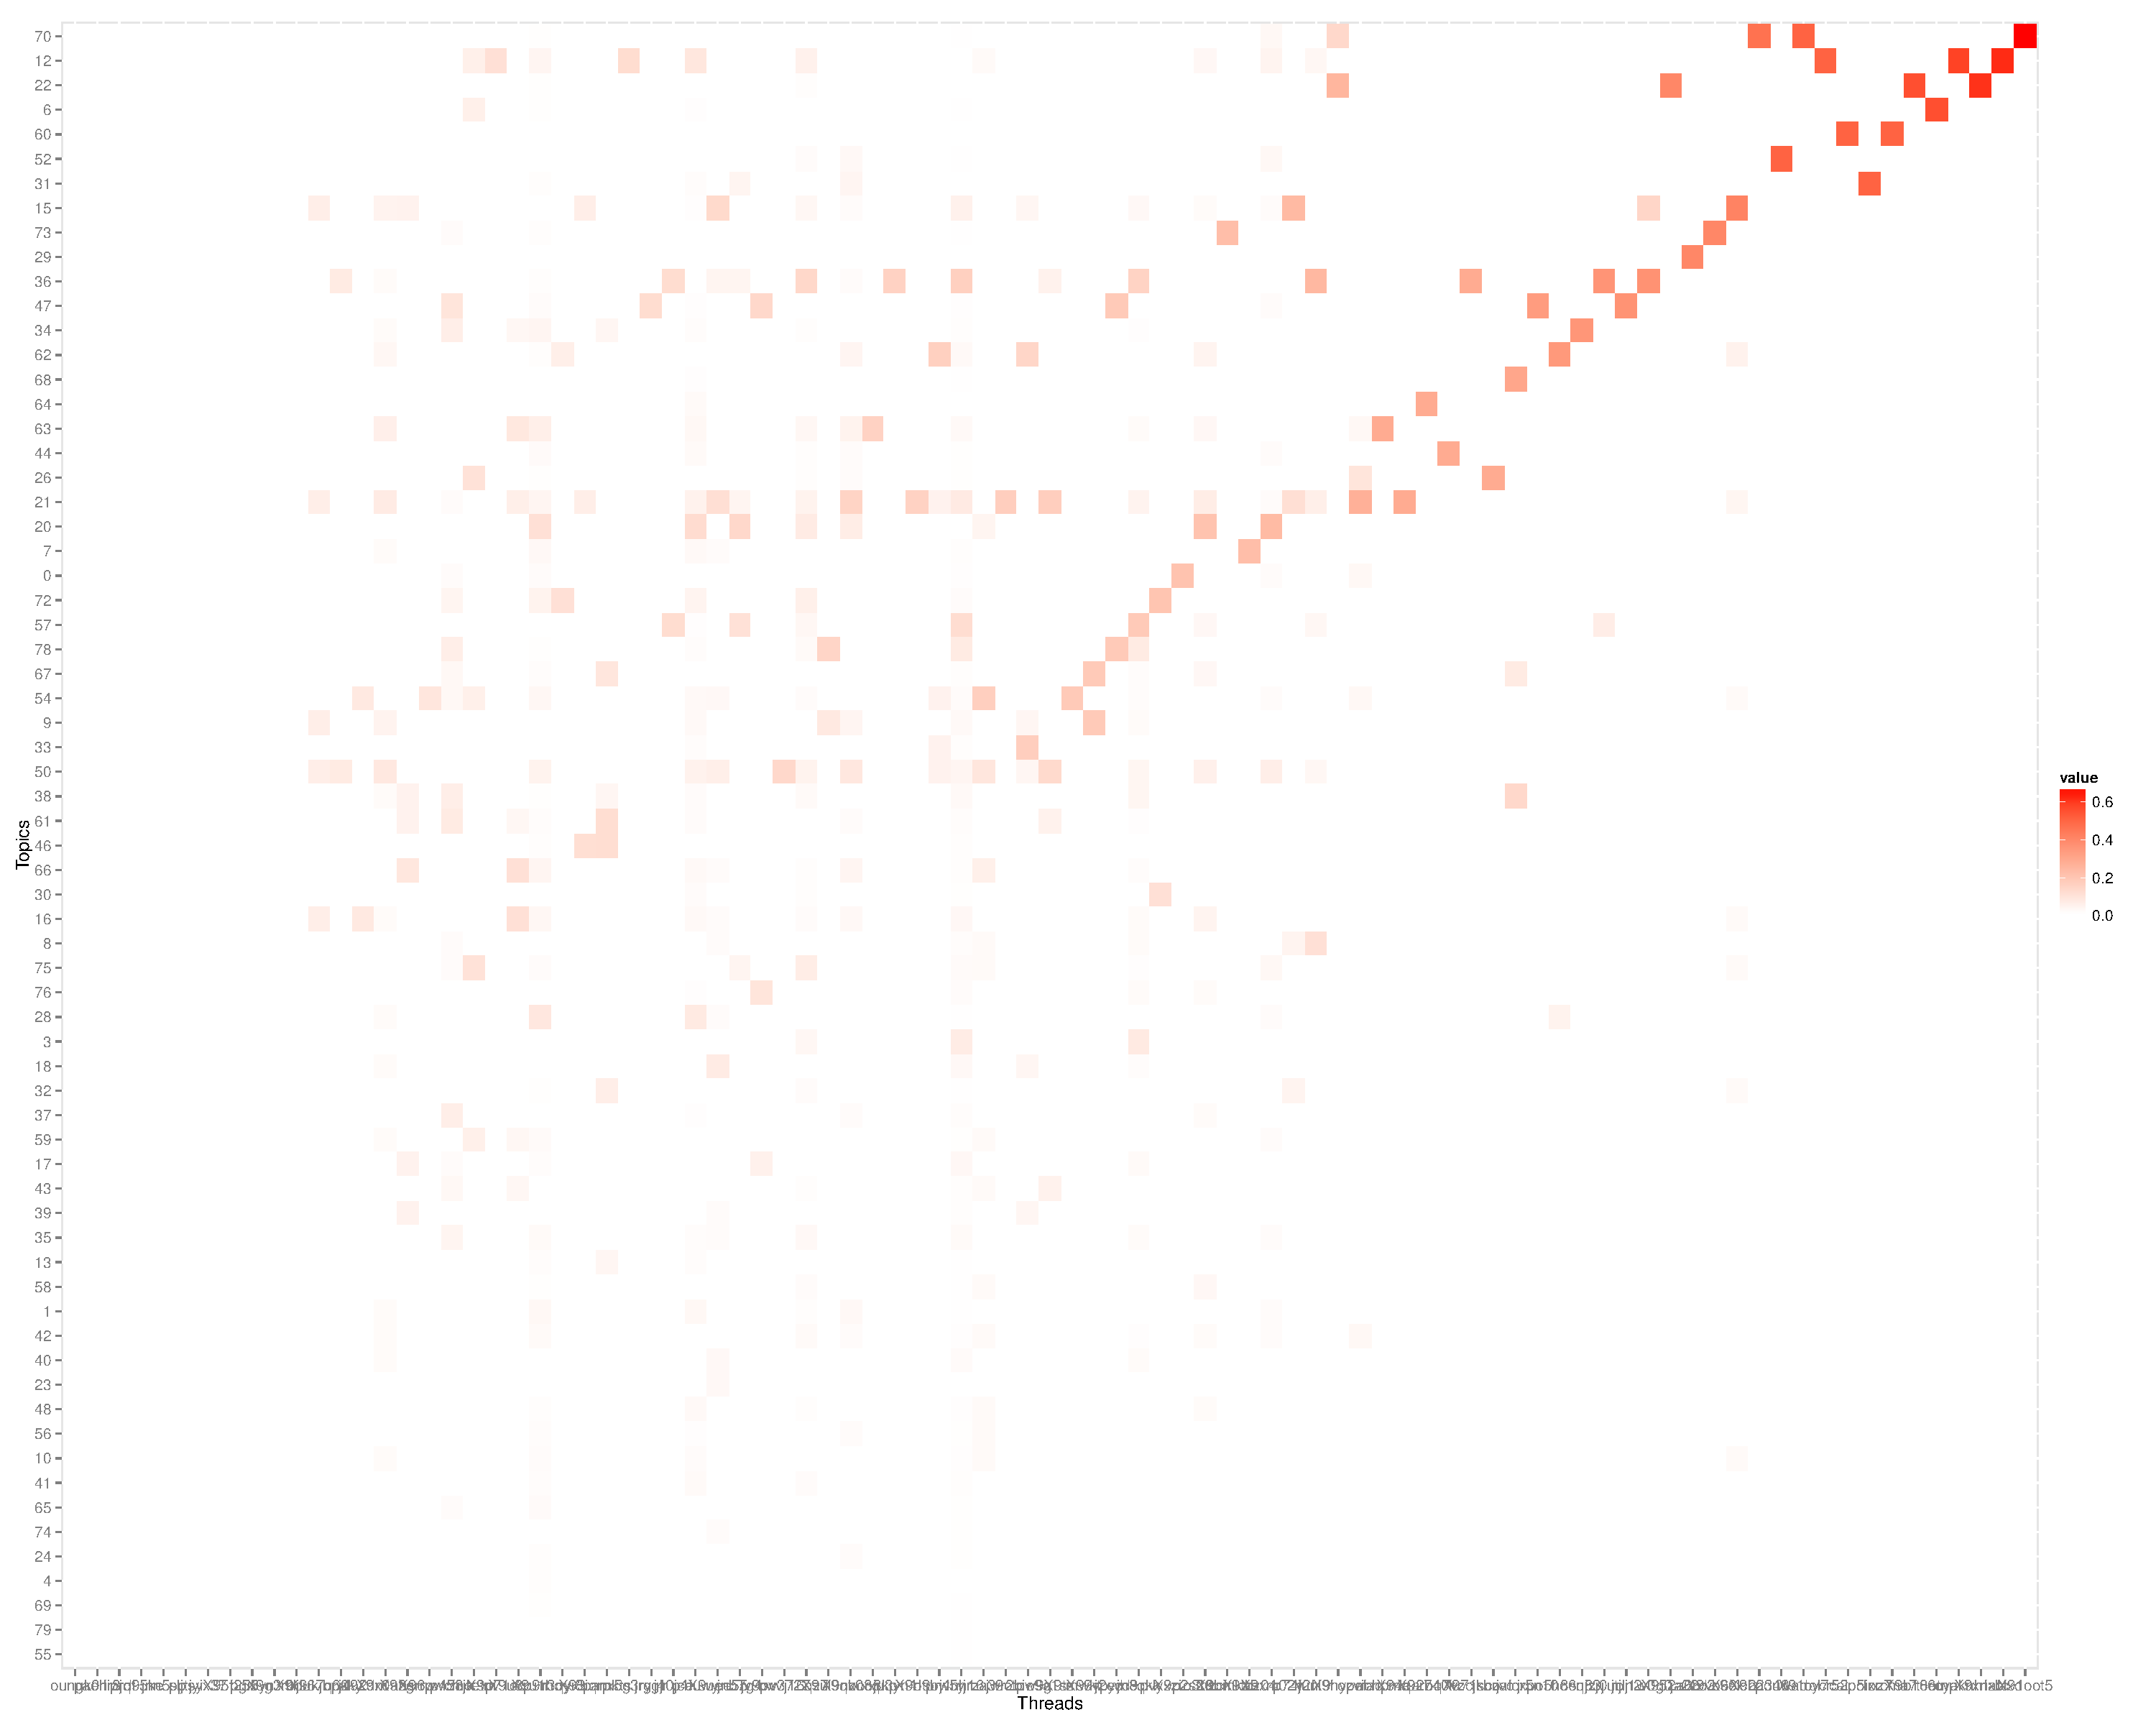
\includegraphics[width=9.5cm]{./imgs/DT_gg_heat.pdf}
  \end{center}
\end{frame}

\begin{frame}\frametitle{When we talk about texting and driving, we talk about \ldots}
\begin{center}
{\Large 
\begin{enumerate}
\item Topic 12: poor graphic design
\item Topic 50: fake ids and fake drivers licenses
\item Topic 58: health/accident insurance
\item Topic 62: drunk drivers
\item Topic 64: buses and bus drivers
\item Topic 67: bikes, bike lanes
\item Topic 68: trucks and truck drivers
\end{enumerate}
}
\end{center}
\end{frame}

\begin{frame}
  \begin{center}
    {\Large Thank you!}  \\ [20pt]
    
\includegraphics[width=3cm]{./imgs/logo.png} \\ [15pt]
    \begin{itemize}
    \item Presentation, data, vis. code at: \url{http://github.com/DrSkippy27/Approach-to-Leveraging-Social-Data_2013}
    \end{itemize}
  \end{center}
\end{frame}

\end{document}
